\section{Quantized model}\label{sec:quantized}

After the floating point model we moved towards lower level, performing a
quantization of input values.

To do that we have to fix their dimensions in bits, that will be the same of the
VHDL implementation, after that we have to fix the range of acceptable \(x\),
\(y\) and \(phase\) values so that we can compute the \emph{LSB} value for
\(x\), \(y\) and \(phase\) as shown in \lstref{lst:cordicq}.

\lstinputlisting[language=matlab, label={lst:cordicq},
caption={CORDIC Quantized Model in Matlab
(\code{cordic\_quantized.m}).}]{matlab/quantized/cordic_quantized.m}

The output of this model with the same inputs given to the floating point model
gives us the opportunity to evaluate the quantization error introduced. In
\figref{fig:qerrorradius} we can appreciate the quantization error on the radius
and in \figref{fig:qerrorphase} the quantization error on the phase.


\begin{figure}[htb]
	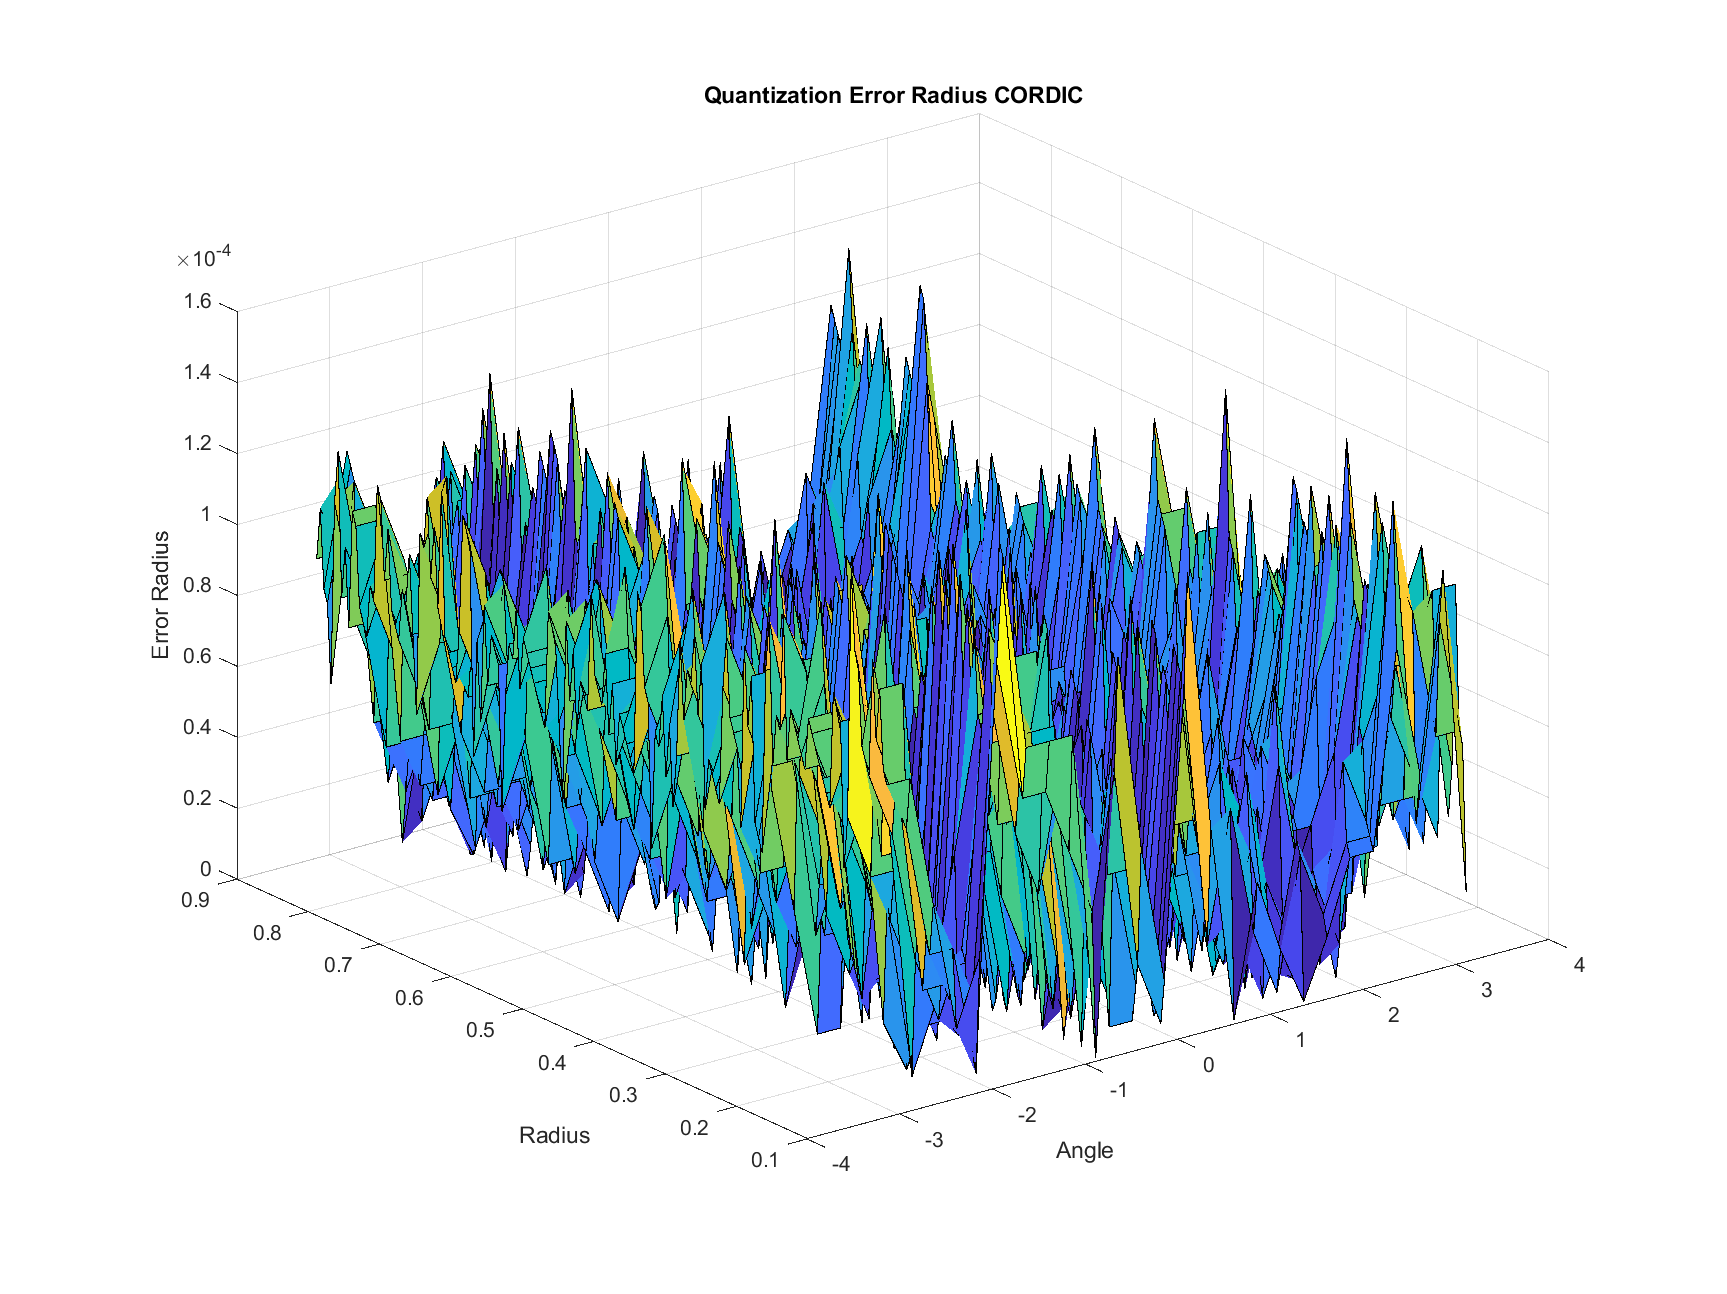
\includegraphics[width=\textwidth]{quant_error_radius}
	\caption{Quantization error Radius}\label{fig:qerrorradius}
\end{figure}
\begin{figure}[htb]
	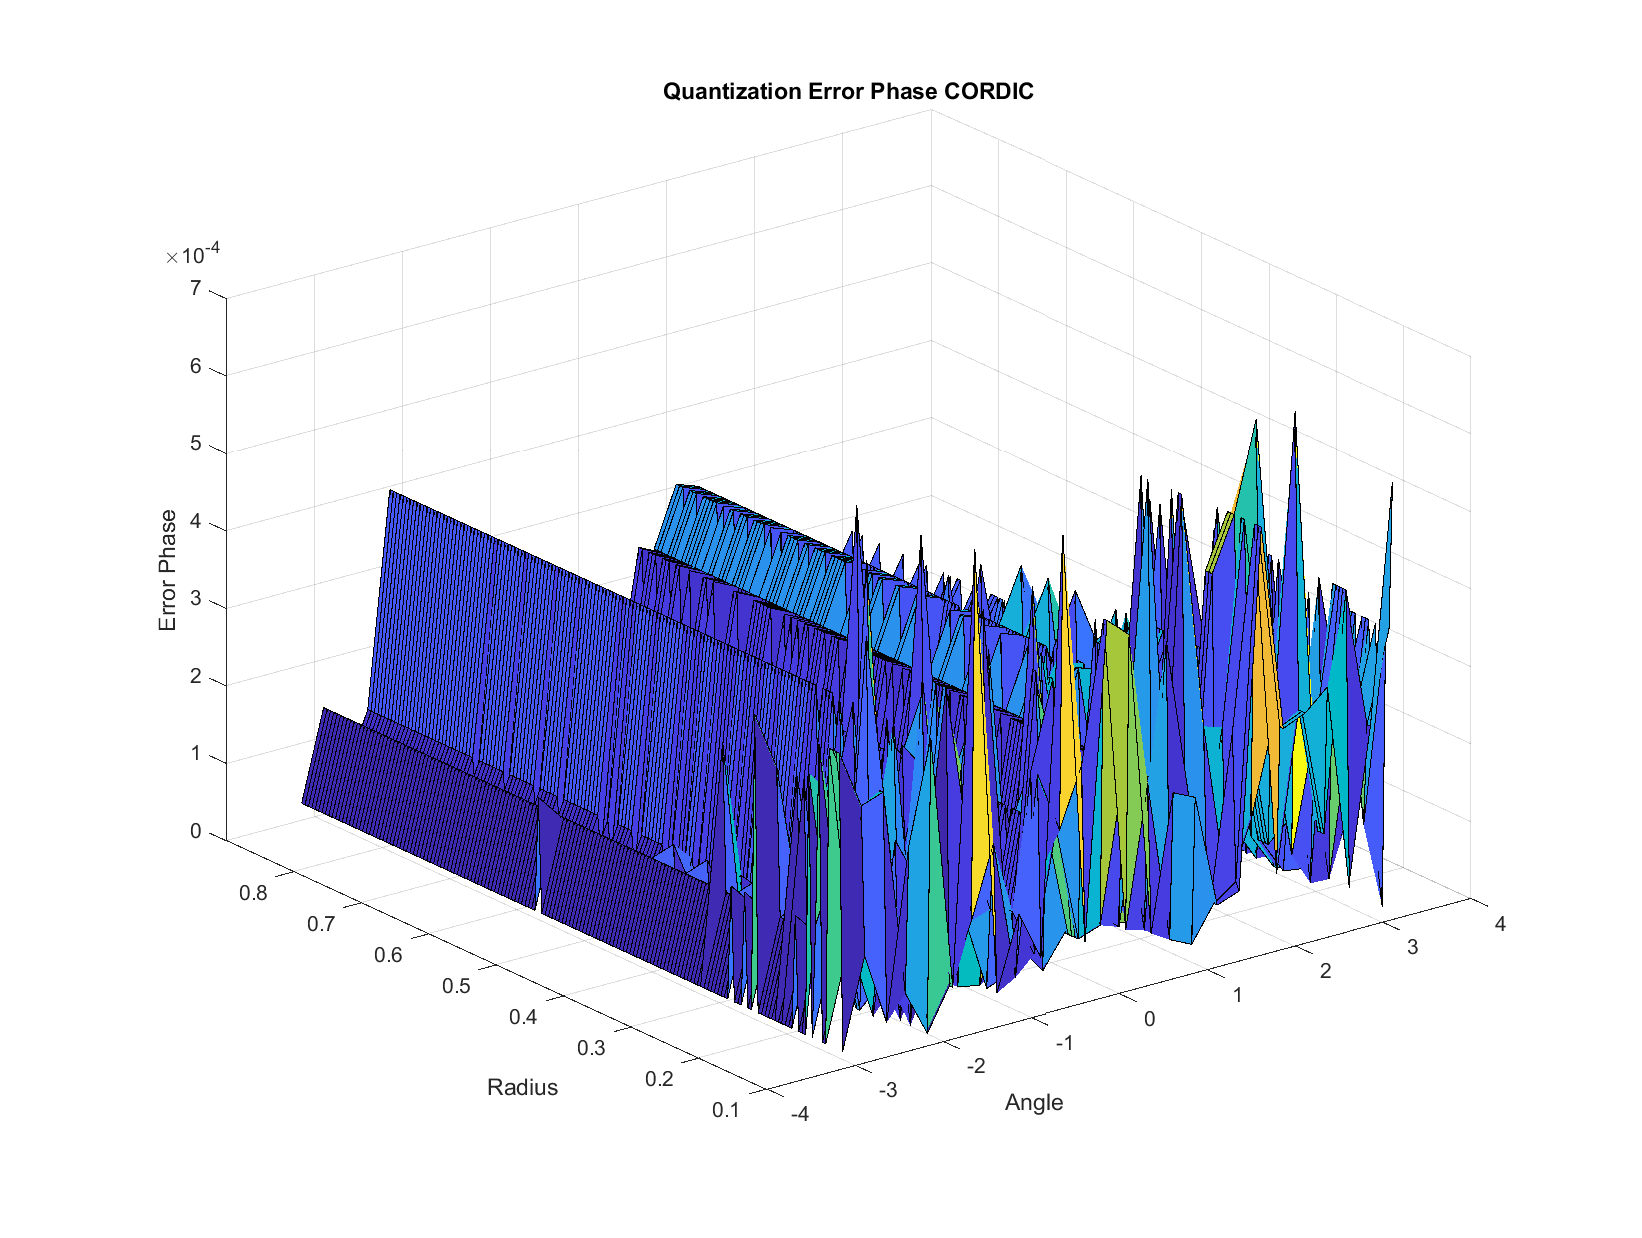
\includegraphics[width=\textwidth]{quant_error_phase}
	\caption{Quantization error Phase}\label{fig:qerrorphase}
\end{figure}
